\documentclass[a4paper]{article}
\usepackage[UTF8]{ctex}
\usepackage{geometry}
\usepackage{graphicx}
\usepackage{url}
\usepackage{multirow}
\usepackage{array}
\usepackage{booktabs}
\usepackage{url}
\usepackage{enumitem}
\usepackage{graphicx}
\usepackage{float}
\usepackage{amssymb}
\usepackage{amsmath}
\usepackage{subfig}
\usepackage{longtable}
\usepackage{color}


\geometry{a4paper, scale=0.78}

% \begin{figure}[H]
%     \centering
%     \includegraphics[width=.55\textwidth]{E.png}
%     \caption{矩阵与列向量的乘法}
%     \label{fig:my_label_1}
% \end{figure}

% \left\{
% \begin{array}{ll}
%       x+2x+z=2 & \\
%       3x+8y+z=12 & \\
%       4y+z=2
% \end{array}
% \right.

\title{Linear classification 03}
\author{Chen Gong}
\date{31 October 2019}

\begin{document}
\maketitle
本小节为线性分类的第三小节,主要推导了线性判别分析算法,也就是Fisher算法。Fisher算法的主要思想是:{\color{red} 类内小,类间大。}这有点类似于,软件过程里的松耦合,高内聚的思想。这个思想转换成数学语言也就是,同一类数据之间的方差要小,不同类数据之间的均值的差距要大。那么,我们对数据的描述如下所示:
\begin{equation}
    X=(x_1, x_2, \cdots, x_N)^T=
    \begin{pmatrix}
    x_1^T \\ 
    x_2^T \\
    \vdots\\
    x_N^T \\
    \end{pmatrix} =
    \begin{pmatrix}
    x_{11} & x_{12} & \dots & x_{1p}\\
    x_{21} & x_{32} & \dots & x_{2p}\\
    \vdots & \vdots & \ddots & \vdots\\
    x_{N1} & x_{N2} & \dots & x_{Np}\\
    \end{pmatrix}_{N\times P}
\end{equation}
\begin{equation}
    Y=
    \begin{pmatrix}
    y_1 \\ 
    y_2 \\
    \vdots\\
    y_N \\
    \end{pmatrix}_{N\times 1}
\end{equation}

那么,我们的数据集可以记为$\left\{ (x_i,y_i) \right\}_{i=1}^N$,其中,$x_i \in \mathbb{R}^p$,$y_i\in\{+1,-1\}$,且$\{y=+1\}$为$C_1$类,且$\{y=-1\}$为$C_2$类。那么,$X_{c_1}$被定义为$\left\{ x_i|y_i=+1 \right\}$,$X_{c_2}$被定义为$\left\{ x_i|y_i=-1 \right\}$。所以,很显然可以得到$|X_{c_1}|=N_1$,$|X_{c_2}|=N_2$,并且$N_1+N_2=N$。

\section{Fisher线性判别分析}
\begin{figure}[H]
    \centering
    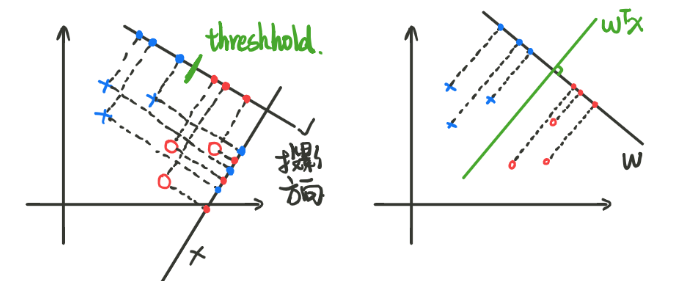
\includegraphics[width=.55\textwidth]{微信图片_20191031095624.png}
    \caption{Fisher线性判别分析模型图}
    \label{fig:my_label_1}
\end{figure}

在左图中,我们设置了两个投影方向,很显然上面那个投影方向可以更好的将两个点之间分开。我们可以在投影方向上找一个点作为两个类别的分界点,也就是阈值(Threshhold)。首先,我们先引入一个有关投影算法的小知识。

\subsection{投影算法}
首先,我们需要设定一个投影向量$w$,为了保险起见,对这个投影向量$w$作出约束,令$||w||=1$。那么,在空间中的一个数据点,也就是一个向量,在投影向量上的投影长度可以表述为:
\begin{equation}
    x_i\cdot w = |x_i||w|\cos{\theta}=|x_i|\cos{\theta}=\triangle
\end{equation}

\subsection{Fisher判别分析的损失函数表达式}
在这个部分,主要是要得出Fisher判别分析的损失函数表达式求法。对于,投影的平均值和方差,我们可以分别表述为:
\begin{gather}
    \Bar{z}=\frac{1}{N}\sum_{i=1}^{N}z_i = \frac{1}{N}\sum_{i=1}^{N}w^Tx_i \\
    S_z=\frac{1}{N}\sum_{i=1}^N(z_i-\Bar{z})(z_i-\Bar{z})^T
\end{gather}

那么对于第一类分类点$X_{c_1}$和第二类分类点$X_{c_2}$可以表述为:
\begin{equation}
    C_1:\qquad \Bar{z_1}= \frac{1}{N_1}\sum_{i=1}^{N_1}w^Tx_i \qquad S_1 =\frac{1}{N_1}\sum_{i=1}^N(z_i-\Bar{z_1})(z_i-\Bar{z_1})^T
\end{equation}
\begin{equation}
    C_2:\qquad \Bar{z_2}= \frac{1}{N_2}\sum_{i=1}^{N_2}w^Tx_i \qquad S_2 =\frac{1}{N_2}\sum_{i=1}^N(z_i-\Bar{z_2})(z_i-\Bar{z_2})^T
\end{equation}

那么类间的距离我们可以定义为:$(\Bar{z_1}-\Bar{z_2})^2$,
类内的距离被我们定义为$S_1+S_2$。那么我们的目标函数Target Function $\mathcal{J}(w)$,可以被定义为:
\begin{equation}
    \mathcal{J}(w) = \frac{(\Bar{z_1}-\Bar{z_2})^2}{S_1+S_2}
\end{equation}

因为,我们的目的是使方差越小越好,均值之间的差越大越好。

\subsection{损失函数表达式的化简}
\subsubsection{$(\Bar{z_1}-\Bar{z_2})^2$}
分子的化简过程如下所示:
\begin{equation}
    \begin{split}
        (\Bar{z_1}-\Bar{z_2})^2 
        = & \left( \frac{1}{N_1}\sum_{i=1}^{N_1}w^Tx_i - \frac{1}{N_2}\sum_{i=1}^{N_2}w^Tx_i \right)^2 \\
        = & \left( w^T(\frac{1}{N_1}\sum_{i=1}^{N_1}x_i - \frac{1}{N_2}\sum_{i=1}^{N_2}x_i ) \right)^2 \\
        = & \left( w^T(\Bar{X}_{c_1} - \Bar{X}_{c_2}) \right)^2 \\
        = & w^T(\Bar{X}_{c_1} - \Bar{X}_{c_2})(\Bar{X}_{c_1} - \Bar{X}_{c_2})^Tw \\
    \end{split}
\end{equation}

\subsubsection{$S_1+S_2$}
分母的化简过程如下所示:
\begin{equation}
    \begin{split}
        S_1 = & \frac{1}{N_1}\sum_{i=1}^N(z_i-\Bar{z}_1)(z_i-\Bar{z}_1)^T \\
        = & \frac{1}{N_1}\sum_{i=1}^N(w^Tx_i-\frac{1}{N_1}\sum_{i=1}^{N_1}w^Tx_i)(w^Tx_i-\frac{1}{N_1}\sum_{i=1}^{N_1}w^Tx_i)^T \\
        = & w^T\frac{1}{N_1}\sum_{i=1}^N(x_i-\frac{1}{N_1}\sum_{i=1}^{N_1}x_i)(x_i-\frac{1}{N_1}\sum_{i=1}^{N_1}x_i)^Tw \\
        = & w^TS_{c_1}w \\
    \end{split}
\end{equation}

同理可得,
\begin{equation}
    S_1 = w^TS_{c_2}w
\end{equation}


所以,
\begin{equation}
    S_1+S_2=w^T(S_{c_1}+S_{c_2})w
\end{equation}

\subsubsection{$\mathcal{J}(w)$的最简表达形式}
\begin{equation}
    \mathcal{J}(w)=\frac{w^T(\Bar{X}_{c_1} - \Bar{X}_{c_2})(\Bar{X}_{c_1} - \Bar{X}_{c_2})^Tw}{w^T(S_{c_1}+S_{c_2})w}
\end{equation}

令$S_b$为between-class类间方差,$S_w$为within-class,也就是类内方差。那么有
\begin{equation}
    S_b = (\Bar{X}_{c_1} - \Bar{X}_{c_2})(\Bar{X}_{c_1} - \Bar{X}_{c_2})^T \qquad S_w = (S_{c_1}+S_{c_2}) 
\end{equation}

于是,我们可以得到进一步化简的表达式;
\begin{equation}
    \mathcal{J}(w)=\frac{w^TS_bw}{w^TS_ww}
\end{equation}

\subsection{损失函数$\mathcal{J}(w)$的梯度}
为了方便求导,我们令$\mathcal{J}(w)=(w^TS_bw)(w^TS_ww)^{-1}$。
\begin{equation}
    \begin{split}
        \frac{\partial \mathcal{J}(w)}{\partial w} = 2S_bw(w^TS_ww)^{-1} + & (-1)(w^TS_bw)(w^TS_ww)^{-2}(2)S_ww = 0 \\
        S_bw(w^TS_ww)^{-1} = & (w^TS_bw)(w^TS_ww)^{-2}S_ww\\
    \end{split}
\end{equation}

显然,$w$的维度是$p\times 1$,$w^T$的维度是$1 \times p$,$S_w$的维度是$p\times p$,所以,$w^TS_ww$是一个实数,同理 可得,$w^TS_ww$是一个实数所以,可以得到
\begin{equation}
    \begin{split}
        S_bw = & (w^TS_bw)(w^TS_ww)^{-1}S_ww \\
        S_bw = & \frac{(w^TS_bw)}{(w^TS_ww)}S_ww
    \end{split}
\end{equation}

我们主要是求得梯度的方向,大小不是很重要了。所以,我们可得
\begin{equation}
    w = \frac{(w^TS_bw)}{(w^TS_ww)}S_b^{-1}S_ww \propto S_b^{-1}S_ww
\end{equation}
\begin{equation}
    S_ww =  (\Bar{X}_{c_1} - \Bar{X}_{c_2})(\Bar{X}_{c_1} - \Bar{X}_{c_2})^Tw
\end{equation}

而$(\Bar{X}_{c_1} - \Bar{X}_{c_2})^Tw$是一个实数,所以汇总可得
\begin{equation}
    S_b^{-1}S_ww \propto S_w^{-1}(\Bar{X}_{c_1} - \Bar{X}_{c_2})
\end{equation}

那么,我们就可以求得梯度的方向为$S_w^{-1}(\Bar{X}_{c_1} - \Bar{X}_{c_2})$。如果,$S_w^{-1}$是一个各向同性的对角矩阵,那么$S^{-1}\propto I$。所以,$w\propto (\Bar{X}_{c_1} - \Bar{X}_{c_2})$。既然,求得了梯度的方向,其实梯度的大小就不重要的。

\end{document}
